\documentclass[convert={density=300,size=400x300,outext=.png}]{standalone}
\usepackage{tikz}

\thispagestyle{empty}

\begin{document}
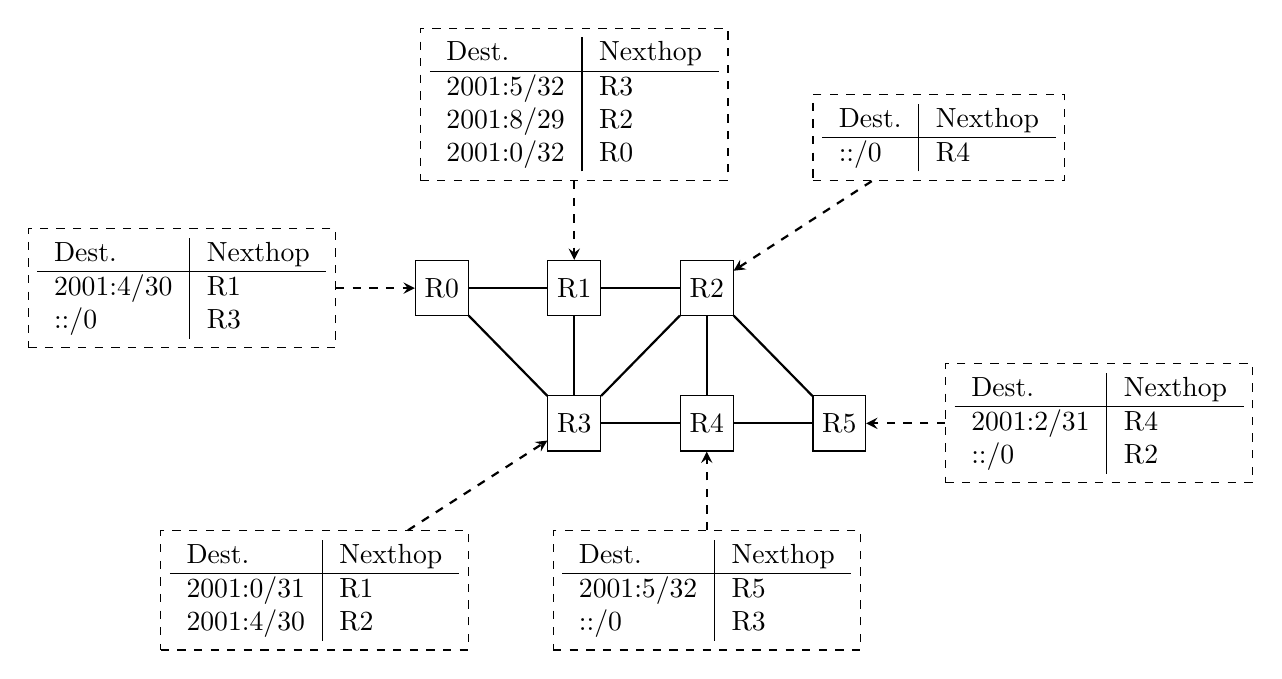
\begin{tikzpicture}
  \usetikzlibrary{positioning,matrix,arrows}
 

        \tikzstyle{arrow} = [thick,->,>=stealth]
        \tikzset{router/.style = {rectangle, draw, text centered, minimum height=2em}, }
        \tikzset{host/.style = {circle, draw, text centered, minimum height=2em}, }
        \tikzset{ftable/.style={rectangle, dashed, draw} }

        \node[router] (R0) {R0};
        \node[router, right=of R0] (R1) { R1 };
        \node[ftable, above =of R1] (FR1) { \begin{tabular}{l|l} 
        Dest. & Nexthop \\
        \hline 
        2001:5/32 & R3 \\
        2001:8/29 & R2 \\
        2001:0/32 & R0 \\
        \end{tabular}};
        \node[router,right=of R1] (R2) {R2};
        \node[ftable, above right=of R2] (FR2) { \begin{tabular}{l|l} 
        Dest. & Nexthop \\
        \hline 
        ::/0 & R4 \\
        \end{tabular}};
        \node[router,below=of R1] (R3) {R3};
        \node[ftable,below left=of R3] (FR3) { \begin{tabular}{l|l} 
        Dest. & Nexthop \\
        \hline 
        2001:0/31  & R1 \\
        2001:4/30 & R2 \\        
        \end{tabular}\\};
        \node[router,below=of R2] (R4) {R4};
        \node[ftable,below =of R4] (FR4) { \begin{tabular}{l|l} 
        Dest. & Nexthop \\
        \hline 
        2001:5/32 & R5 \\
        ::/0 & R3 \\        
        \end{tabular}\\};
        \node[router, right=of R4] (R5) {R5};
        \node[ftable, right =of R5] (FR5) { \begin{tabular}{l|l} 
        Dest. & Nexthop \\
        \hline 
        2001:2/31 & R4 \\
        ::/0 & R2      \\        
        \end{tabular}};
        \node[ftable, left =of R0] (FR0) { \begin{tabular}{l|l} 
        Dest. & Nexthop \\
        \hline 
        2001:4/30 & R1 \\
        ::/0 & R3      \\        
        \end{tabular}};
        
        \path[draw,thick]
        (R0) edge (R1)
        (R0) edge (R3) 
        (R1) edge (R2) 
        (R2) edge (R3) 
        (R1) edge (R3) 
        (R4) edge (R3) 
        (R2) edge (R4)
        (R2) edge (R5)
        (R4) edge (R5); 

        \draw[arrow, dashed] (FR0) -- (R0); 
        \draw[arrow, dashed] (FR1) -- (R1); 
        \draw[arrow, dashed] (FR4) -- (R4); 
        \draw[arrow, dashed] (FR2) -- (R2); 
        \draw[arrow, dashed] (FR3) -- (R3);
        \draw[arrow, dashed] (FR5) -- (R5); 


\end{tikzpicture}
\end{document}
